%!TEX root = ../thesis.tex

\section{テストフェーズ}
提案手法におけるテストフェーズでは\figref{Fig:suggest_test_phase}で示すように, 従来手法のシステムから新たに目標方向を学習器の入力へ追加した. なお, テストフェーズも学習フェーズと同様に, 地図を用いたルールベース制御器から目標方向を生成している. 
\par
最終的には, 目的地までカメラ画像のみで自律移動させることを目標としているため, 目標方向を画像から自動的に作成する仕組みが必要となるが, それは今後の課題として, 本論文では議論しない.
% そのため, 以下のようなROSパッケージを作成している\cite{weighted_graph}.

% \begin{itemize}
%      \item GUI上で目的地(ノード)を設定すると, ダイクストラ法でノード間の距離を考慮した経路探索を行う. その後, 経由するノードの位置関係から目標方向を自動生成し, 同時にカメラ画像からノードの場所検出を行い, 適切な目標方向に切り替える.
% \end{itemize}

% figに動作の様子を示す. 
\par
カメラ画像と目標方向を入力した学習器の出力による自律移動をさせる際に, 目標方向によって任意の経路を選択する.

\vspace{1cm}

\begin{figure}[hbtp]
  \centering
 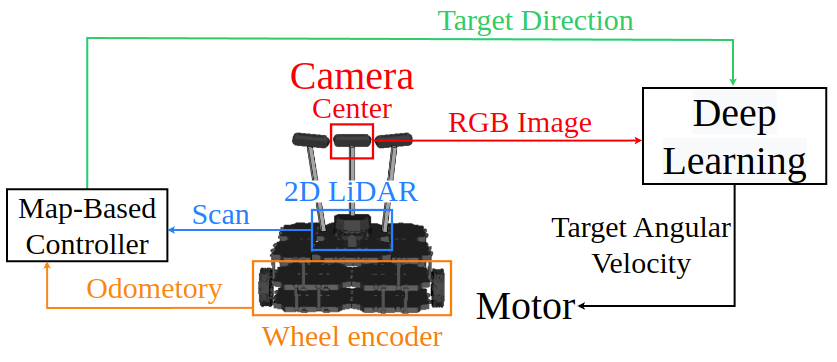
\includegraphics[keepaspectratio, scale=0.46]
      {images/suggest_test_phase.png}
 \caption{Learning phase system of proposed method}
 \label{Fig:suggest_test_phase}
\end{figure}

% \subsubsection{etc...}
\newpage
